\hypertarget{dbprim_8h}{
\section{dbprim.h File Reference}
\label{dbprim_8h}\index{dbprim.h@{dbprim.h}}
}


\subsection{Detailed Description}
This header file contains the necessary structures, \#define's, and function declarations to make use of the Database Primitives library.

Definition in file \hyperlink{dbprim_8h-source}{dbprim.h}.

{\tt \#include $<$dbprim/dbprim\_\-err.h$>$}\par
{\tt \#include $<$dbprim/dbprim\_\-version.h$>$}\par


Include dependency graph for dbprim.h:\begin{figure}[H]
\begin{center}
\leavevmode
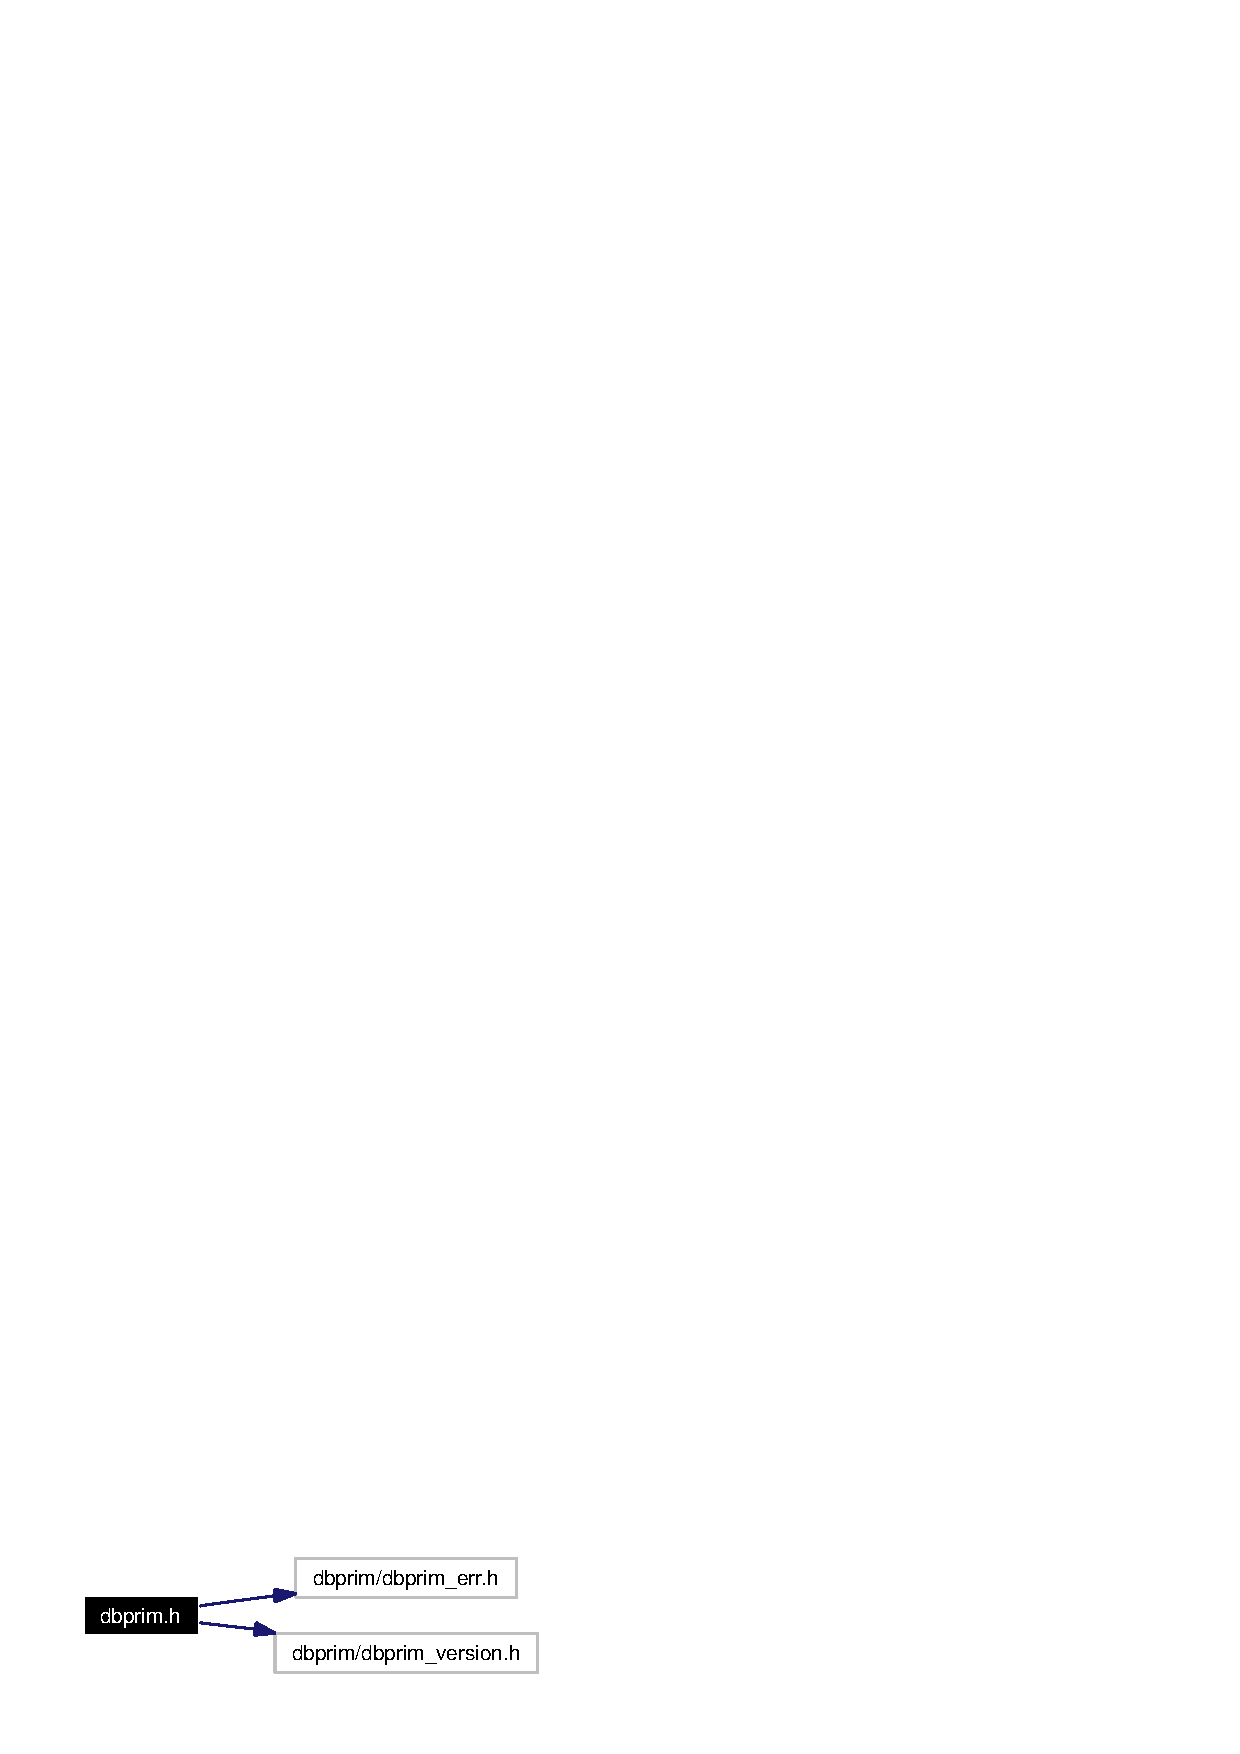
\includegraphics[width=131pt]{dbprim_8h__incl}
\end{center}
\end{figure}


This graph shows which files directly or indirectly include this file:\begin{figure}[H]
\begin{center}
\leavevmode
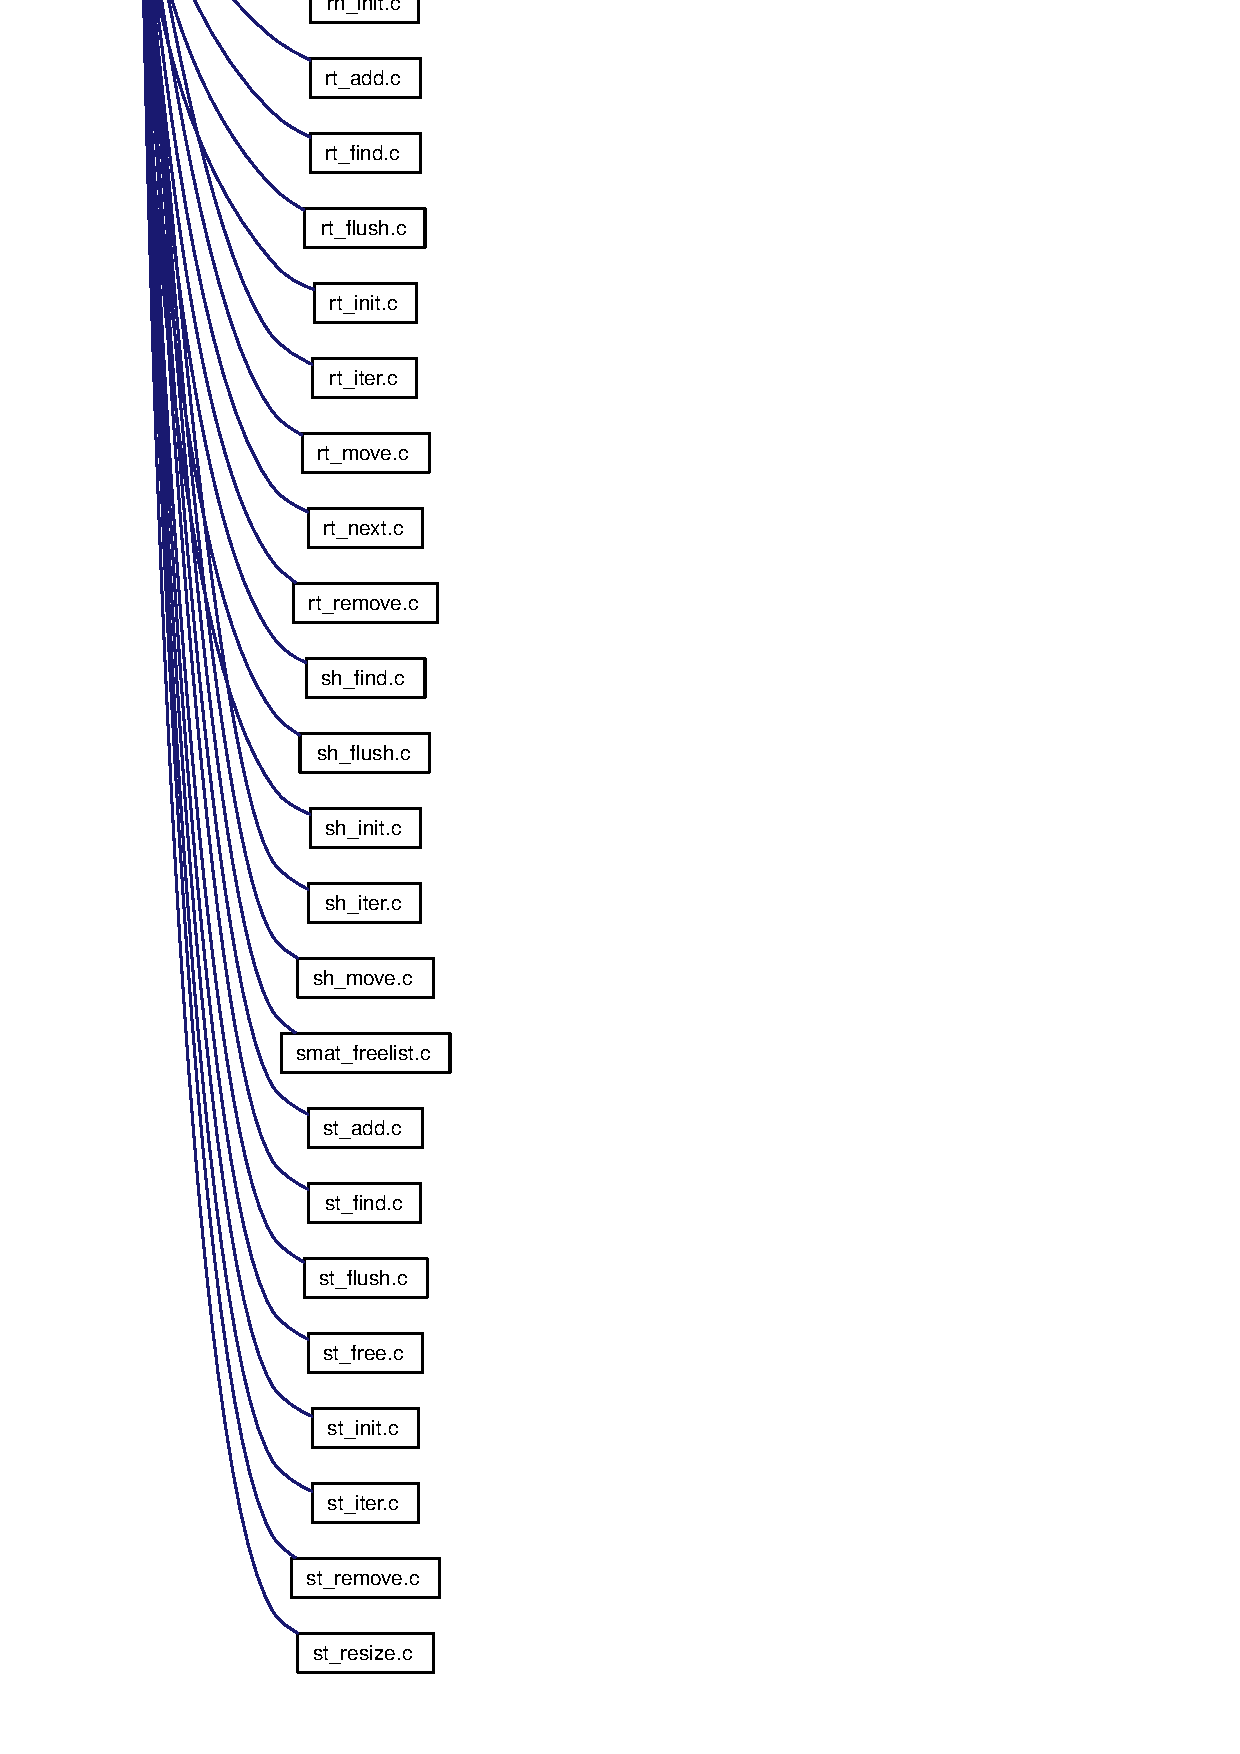
\includegraphics[width=111pt]{dbprim_8h__dep__incl}
\end{center}
\end{figure}
\subsection*{Data Structures}
\begin{CompactItemize}
\item 
struct \hyperlink{struct__db__key__s}{\_\-db\_\-key\_\-s}
\begin{CompactList}\small\item\em Database key structure. \item\end{CompactList}\item 
struct \hyperlink{struct__link__head__s}{\_\-link\_\-head\_\-s}
\begin{CompactList}\small\item\em Linked list head structure. \item\end{CompactList}\item 
struct \hyperlink{struct__link__elem__s}{\_\-link\_\-elem\_\-s}
\begin{CompactList}\small\item\em Linked list element structure. \item\end{CompactList}\item 
struct \hyperlink{struct__hash__table__s}{\_\-hash\_\-table\_\-s}
\begin{CompactList}\small\item\em Hash table structure. \item\end{CompactList}\item 
struct \hyperlink{struct__hash__entry__s}{\_\-hash\_\-entry\_\-s}
\begin{CompactList}\small\item\em Hash table entry structure. \item\end{CompactList}\item 
struct \hyperlink{struct__smat__table__s}{\_\-smat\_\-table\_\-s}
\begin{CompactList}\small\item\em Sparse matrix table structure. \item\end{CompactList}\item 
struct \hyperlink{struct__smat__head__s}{\_\-smat\_\-head\_\-s}
\begin{CompactList}\small\item\em Sparse matrix list head structure. \item\end{CompactList}\item 
struct \hyperlink{struct__smat__entry__s}{\_\-smat\_\-entry\_\-s}
\begin{CompactList}\small\item\em Sparse matrix entry structure. \item\end{CompactList}\item 
struct \hyperlink{struct__rb__tree__s}{\_\-rb\_\-tree\_\-s}
\begin{CompactList}\small\item\em Red-black tree structure. \item\end{CompactList}\item 
struct \hyperlink{struct__rb__node__s}{\_\-rb\_\-node\_\-s}
\begin{CompactList}\small\item\em Red-black tree node structure. \item\end{CompactList}\end{CompactItemize}
\subsection*{Defines}
\begin{CompactItemize}
\item 
\#define \hyperlink{dbprim_8h_a0}{DBPRIM\_\-BEGIN\_\-C\_\-DECLS}
\begin{CompactList}\small\item\em Begin declaration in C namespace. \item\end{CompactList}\item 
\#define \hyperlink{dbprim_8h_a1}{DBPRIM\_\-END\_\-C\_\-DECLS}
\begin{CompactList}\small\item\em End declaration in C namespace. \item\end{CompactList}\item 
\#define \hyperlink{group__dbprim_ga1}{DB\_\-KEY\_\-INIT}(key, size)
\begin{CompactList}\small\item\em Database key static initializer. \item\end{CompactList}\item 
\#define \hyperlink{group__dbprim_ga2}{dk\_\-key}(key)
\begin{CompactList}\small\item\em Database key accessor macro. \item\end{CompactList}\item 
\#define \hyperlink{group__dbprim_ga3}{dk\_\-len}(key)
\begin{CompactList}\small\item\em Database key length accessor macro. \item\end{CompactList}\item 
\#define \hyperlink{group__dbprim_ga4}{DB\_\-FLAG\_\-REVERSE}
\begin{CompactList}\small\item\em Reverse flag. \item\end{CompactList}\item 
\#define \hyperlink{group__dbprim__link_ga13}{LINK\_\-HEAD\_\-MAGIC}
\begin{CompactList}\small\item\em Linked list head magic number. \item\end{CompactList}\item 
\#define \hyperlink{group__dbprim__link_ga14}{LINK\_\-HEAD\_\-INIT}(extra)
\begin{CompactList}\small\item\em Linked list head static initializer. \item\end{CompactList}\item 
\#define \hyperlink{group__dbprim__link_ga15}{ll\_\-verify}(list)
\begin{CompactList}\small\item\em Linked list head verification macro. \item\end{CompactList}\item 
\#define \hyperlink{group__dbprim__link_ga16}{ll\_\-count}(list)
\begin{CompactList}\small\item\em Linked list count. \item\end{CompactList}\item 
\#define \hyperlink{group__dbprim__link_ga17}{ll\_\-first}(list)
\begin{CompactList}\small\item\em First element in linked list. \item\end{CompactList}\item 
\#define \hyperlink{group__dbprim__link_ga18}{ll\_\-last}(list)
\begin{CompactList}\small\item\em Last element in a linked list. \item\end{CompactList}\item 
\#define \hyperlink{group__dbprim__link_ga19}{ll\_\-extra}(list)
\begin{CompactList}\small\item\em Extra pointer data in a linked list. \item\end{CompactList}\item 
\#define \hyperlink{group__dbprim__link_ga20}{LINK\_\-ELEM\_\-MAGIC}
\begin{CompactList}\small\item\em Linked list element magic number. \item\end{CompactList}\item 
\#define \hyperlink{group__dbprim__link_ga21}{LINK\_\-ELEM\_\-INIT}(obj)
\begin{CompactList}\small\item\em Linked list element static initializer. \item\end{CompactList}\item 
\#define \hyperlink{group__dbprim__link_ga22}{le\_\-verify}(element)
\begin{CompactList}\small\item\em Linked list element verification macro. \item\end{CompactList}\item 
\#define \hyperlink{group__dbprim__link_ga23}{le\_\-next}(elem)
\begin{CompactList}\small\item\em Linked list element next pointer. \item\end{CompactList}\item 
\#define \hyperlink{group__dbprim__link_ga24}{le\_\-prev}(elem)
\begin{CompactList}\small\item\em Linked list element previous pointer. \item\end{CompactList}\item 
\#define \hyperlink{group__dbprim__link_ga25}{le\_\-object}(elem)
\begin{CompactList}\small\item\em Linked list element object pointer. \item\end{CompactList}\item 
\#define \hyperlink{group__dbprim__link_ga26}{le\_\-head}(elem)
\begin{CompactList}\small\item\em Linked list element head pointer. \item\end{CompactList}\item 
\#define \hyperlink{group__dbprim__link_ga27}{le\_\-flags}(elem)
\begin{CompactList}\small\item\em Linked list element flags. \item\end{CompactList}\item 
\#define \hyperlink{group__dbprim__hash_ga22}{HASH\_\-TABLE\_\-MAGIC}
\begin{CompactList}\small\item\em Hash table magic number. \item\end{CompactList}\item 
\#define \hyperlink{group__dbprim__hash_ga23}{HASH\_\-FLAG\_\-AUTOGROW}
\begin{CompactList}\small\item\em Flag permitting a hash table to automatically grow. \item\end{CompactList}\item 
\#define \hyperlink{group__dbprim__hash_ga24}{HASH\_\-FLAG\_\-AUTOSHRINK}
\begin{CompactList}\small\item\em Flag permitting a hash table to automatically shrink. \item\end{CompactList}\item 
\#define \hyperlink{group__dbprim__hash_ga25}{HASH\_\-FLAG\_\-MASK}
\begin{CompactList}\small\item\em Hash table flags that may be set by the user. \item\end{CompactList}\item 
\#define \hyperlink{dbprim_8h_a25}{HASH\_\-FLAG\_\-FREEZE}
\begin{CompactList}\small\item\em Flag indicating hash table is frozen. \item\end{CompactList}\item 
\#define \hyperlink{group__dbprim__hash_ga26}{HASH\_\-TABLE\_\-INIT}(flags, func, comp, resize, extra)
\begin{CompactList}\small\item\em Hash table static initializer. \item\end{CompactList}\item 
\#define \hyperlink{group__dbprim__hash_ga27}{ht\_\-verify}(table)
\begin{CompactList}\small\item\em Hash table verification macro. \item\end{CompactList}\item 
\#define \hyperlink{group__dbprim__hash_ga28}{ht\_\-flags}(table)
\begin{CompactList}\small\item\em Hash table flags. \item\end{CompactList}\item 
\#define \hyperlink{group__dbprim__hash_ga29}{ht\_\-frozen}(table)
\begin{CompactList}\small\item\em Determine if a hash table is frozen. \item\end{CompactList}\item 
\#define \hyperlink{group__dbprim__hash_ga30}{ht\_\-modulus}(table)
\begin{CompactList}\small\item\em Hash table modulus. \item\end{CompactList}\item 
\#define \hyperlink{group__dbprim__hash_ga31}{ht\_\-count}(table)
\begin{CompactList}\small\item\em Hash table count. \item\end{CompactList}\item 
\#define \hyperlink{group__dbprim__hash_ga32}{ht\_\-func}(table)
\begin{CompactList}\small\item\em Hash table hash function. \item\end{CompactList}\item 
\#define \hyperlink{group__dbprim__hash_ga33}{ht\_\-comp}(table)
\begin{CompactList}\small\item\em Hash table comparison function. \item\end{CompactList}\item 
\#define \hyperlink{group__dbprim__hash_ga34}{ht\_\-rsize}(table)
\begin{CompactList}\small\item\em Hash table resize callback function. \item\end{CompactList}\item 
\#define \hyperlink{group__dbprim__hash_ga35}{ht\_\-extra}(table)
\begin{CompactList}\small\item\em Extra pointer data in a hash table. \item\end{CompactList}\item 
\#define \hyperlink{group__dbprim__hash_ga36}{ht\_\-size}(table)
\begin{CompactList}\small\item\em Hash table memory size. \item\end{CompactList}\item 
\#define \hyperlink{group__dbprim__hash_ga37}{HASH\_\-ENTRY\_\-MAGIC}
\begin{CompactList}\small\item\em Hash table entry magic number. \item\end{CompactList}\item 
\#define \hyperlink{group__dbprim__hash_ga38}{HASH\_\-ENTRY\_\-INIT}(value)
\begin{CompactList}\small\item\em Hash table entry static initializer. \item\end{CompactList}\item 
\#define \hyperlink{group__dbprim__hash_ga39}{he\_\-verify}(entry)
\begin{CompactList}\small\item\em Hash table entry verification macro. \item\end{CompactList}\item 
\#define \hyperlink{group__dbprim__hash_ga40}{he\_\-link}(entry)
\begin{CompactList}\small\item\em Hash table entry linked list element. \item\end{CompactList}\item 
\#define \hyperlink{group__dbprim__hash_ga41}{he\_\-flags}(entry)
\begin{CompactList}\small\item\em Hash table entry flags. \item\end{CompactList}\item 
\#define \hyperlink{group__dbprim__hash_ga42}{he\_\-table}(entry)
\begin{CompactList}\small\item\em Hash table entry table pointer. \item\end{CompactList}\item 
\#define \hyperlink{group__dbprim__hash_ga43}{he\_\-hash}(entry)
\begin{CompactList}\small\item\em Hash table entry hash value. \item\end{CompactList}\item 
\#define \hyperlink{group__dbprim__hash_ga44}{he\_\-key}(entry)
\begin{CompactList}\small\item\em Hash table entry key pointer. \item\end{CompactList}\item 
\#define \hyperlink{group__dbprim__hash_ga45}{he\_\-value}(entry)
\begin{CompactList}\small\item\em Hash table entry value pointer. \item\end{CompactList}\item 
\#define \hyperlink{group__dbprim__smat_ga32}{\_\-smat\_\-ent}(ent)
\begin{CompactList}\small\item\em Retrieve pointer to sparse matrix entry. \item\end{CompactList}\item 
\#define \hyperlink{group__dbprim__smat_ga33}{SMAT\_\-TABLE\_\-MAGIC}
\begin{CompactList}\small\item\em Sparse matrix table magic number. \item\end{CompactList}\item 
\#define \hyperlink{group__dbprim__smat_ga34}{st\_\-verify}(table)
\begin{CompactList}\small\item\em Sparse matrix table verification macro. \item\end{CompactList}\item 
\#define \hyperlink{group__dbprim__smat_ga35}{st\_\-flags}(table)
\begin{CompactList}\small\item\em Sparse matrix table flags. \item\end{CompactList}\item 
\#define \hyperlink{group__dbprim__smat_ga36}{st\_\-frozen}(table)
\begin{CompactList}\small\item\em Determine if a sparse matrix is frozen. \item\end{CompactList}\item 
\#define \hyperlink{group__dbprim__smat_ga37}{st\_\-modulus}(table)
\begin{CompactList}\small\item\em Sparse matrix table modulus. \item\end{CompactList}\item 
\#define \hyperlink{group__dbprim__smat_ga38}{st\_\-count}(table)
\begin{CompactList}\small\item\em Sparse matrix table count. \item\end{CompactList}\item 
\#define \hyperlink{group__dbprim__hash_ga46}{st\_\-rsize}(table)
\begin{CompactList}\small\item\em Sparse matrix table resize callback function. \item\end{CompactList}\item 
\#define \hyperlink{group__dbprim__smat_ga39}{st\_\-extra}(table)
\begin{CompactList}\small\item\em Extra pointer data in a sparse matrix table. \item\end{CompactList}\item 
\#define \hyperlink{group__dbprim__smat_ga40}{st\_\-size}(table)
\begin{CompactList}\small\item\em Sparse matrix table memory size. \item\end{CompactList}\item 
\#define \hyperlink{group__dbprim__smat_ga41}{SMAT\_\-HEAD\_\-MAGIC}
\begin{CompactList}\small\item\em Sparse matrix list head magic number. \item\end{CompactList}\item 
\#define \hyperlink{group__dbprim__smat_ga42}{SMAT\_\-HEAD\_\-INIT}(elem, object)
\begin{CompactList}\small\item\em Sparse matrix list head static initializer. \item\end{CompactList}\item 
\#define \hyperlink{group__dbprim__smat_ga43}{sh\_\-verify}(head)
\begin{CompactList}\small\item\em Sparse matrix list head verification macro. \item\end{CompactList}\item 
\#define \hyperlink{group__dbprim__smat_ga44}{sh\_\-elem}(head)
\begin{CompactList}\small\item\em Sparse matrix list head element macro. \item\end{CompactList}\item 
\#define \hyperlink{group__dbprim__smat_ga45}{sh\_\-table}(head)
\begin{CompactList}\small\item\em Sparse matrix list head table pointer. \item\end{CompactList}\item 
\#define \hyperlink{group__dbprim__smat_ga46}{sh\_\-frozen}(head)
\begin{CompactList}\small\item\em Determine if a sparse matrix is frozen. \item\end{CompactList}\item 
\#define \hyperlink{group__dbprim__smat_ga47}{sh\_\-count}(head)
\begin{CompactList}\small\item\em Sparse matrix list count. \item\end{CompactList}\item 
\#define \hyperlink{group__dbprim__smat_ga48}{\_\-sh\_\-first}(head)
\begin{CompactList}\small\item\em Access the first element pointer in a \hyperlink{group__dbprim__smat_ga1}{smat\_\-head\_\-t}. \item\end{CompactList}\item 
\#define \hyperlink{group__dbprim__smat_ga49}{sh\_\-first}(head)
\begin{CompactList}\small\item\em First element in sparse matrix list. \item\end{CompactList}\item 
\#define \hyperlink{group__dbprim__smat_ga50}{\_\-sh\_\-last}(head)
\begin{CompactList}\small\item\em Access the last element pointer in a \hyperlink{group__dbprim__smat_ga1}{smat\_\-head\_\-t}. \item\end{CompactList}\item 
\#define \hyperlink{group__dbprim__smat_ga51}{sh\_\-last}(head)
\begin{CompactList}\small\item\em Last element in sparse matrix list. \item\end{CompactList}\item 
\#define \hyperlink{group__dbprim__smat_ga52}{sh\_\-object}(head)
\begin{CompactList}\small\item\em Object represented by a sparse matrix list head. \item\end{CompactList}\item 
\#define \hyperlink{group__dbprim__smat_ga53}{sh\_\-size}(head)
\begin{CompactList}\small\item\em Sparse matrix list memory size. \item\end{CompactList}\item 
\#define \hyperlink{group__dbprim__smat_ga54}{SMAT\_\-ENTRY\_\-MAGIC}
\begin{CompactList}\small\item\em Sparse matrix entry magic number. \item\end{CompactList}\item 
\#define \hyperlink{group__dbprim__smat_ga55}{se\_\-verify}(entry)
\begin{CompactList}\small\item\em Sparse matrix entry verification macro. \item\end{CompactList}\item 
\#define \hyperlink{group__dbprim__smat_ga56}{se\_\-table}(entry)
\begin{CompactList}\small\item\em Sparse matrix entry table. \item\end{CompactList}\item 
\#define \hyperlink{group__dbprim__smat_ga57}{\_\-se\_\-link}(entry)
\begin{CompactList}\small\item\em Sparse matrix entry linked list element. \item\end{CompactList}\item 
\#define \hyperlink{group__dbprim__smat_ga58}{se\_\-flags}(entry)
\begin{CompactList}\small\item\em Sparse matrix entry flags. \item\end{CompactList}\item 
\#define \hyperlink{group__dbprim__smat_ga59}{se\_\-hash}(entry)
\begin{CompactList}\small\item\em Sparse matrix table entry hash value. \item\end{CompactList}\item 
\#define \hyperlink{group__dbprim__smat_ga60}{\_\-se\_\-next}(entry, n)
\begin{CompactList}\small\item\em Access the next element pointer in a \hyperlink{group__dbprim__smat_ga2}{smat\_\-entry\_\-t}. \item\end{CompactList}\item 
\#define \hyperlink{group__dbprim__smat_ga61}{se\_\-next}(entry, n)
\begin{CompactList}\small\item\em Next element in sparse matrix list. \item\end{CompactList}\item 
\#define \hyperlink{group__dbprim__smat_ga62}{\_\-se\_\-prev}(entry, n)
\begin{CompactList}\small\item\em Access the previous element pointer in a \hyperlink{group__dbprim__smat_ga2}{smat\_\-entry\_\-t}. \item\end{CompactList}\item 
\#define \hyperlink{group__dbprim__smat_ga63}{se\_\-prev}(entry, n)
\begin{CompactList}\small\item\em Previous element in sparse matrix list. \item\end{CompactList}\item 
\#define \hyperlink{group__dbprim__smat_ga64}{se\_\-lflags}(entry, n)
\begin{CompactList}\small\item\em Flags associated with an entry in a sparse matrix list. \item\end{CompactList}\item 
\#define \hyperlink{group__dbprim__smat_ga65}{se\_\-object}(entry, n)
\begin{CompactList}\small\item\em Object associated with an entry in a sparse matrix list. \item\end{CompactList}\item 
\#define \hyperlink{group__dbprim__rbtree_ga17}{RB\_\-TREE\_\-MAGIC}
\begin{CompactList}\small\item\em Red-black tree magic number. \item\end{CompactList}\item 
\#define \hyperlink{dbprim_8h_a82}{RBT\_\-FLAG\_\-FREEZE}
\begin{CompactList}\small\item\em Flag indicating red-black tree is frozen. \item\end{CompactList}\item 
\#define \hyperlink{group__dbprim__rbtree_ga18}{RB\_\-TREE\_\-INIT}(comp, extra)
\begin{CompactList}\small\item\em Red-black tree static initializer. \item\end{CompactList}\item 
\#define \hyperlink{group__dbprim__rbtree_ga19}{rt\_\-verify}(tree)
\begin{CompactList}\small\item\em Red-black tree verification macro. \item\end{CompactList}\item 
\#define \hyperlink{group__dbprim__rbtree_ga20}{rt\_\-frozen}(tree)
\begin{CompactList}\small\item\em Determine if a red-black tree is frozen. \item\end{CompactList}\item 
\#define \hyperlink{group__dbprim__rbtree_ga21}{rt\_\-count}(tree)
\begin{CompactList}\small\item\em Red-black tree count. \item\end{CompactList}\item 
\#define \hyperlink{group__dbprim__rbtree_ga22}{rt\_\-root}(tree)
\begin{CompactList}\small\item\em Red-black tree root node. \item\end{CompactList}\item 
\#define \hyperlink{group__dbprim__rbtree_ga23}{rt\_\-comp}(tree)
\begin{CompactList}\small\item\em Red-black tree comparison function. \item\end{CompactList}\item 
\#define \hyperlink{group__dbprim__rbtree_ga24}{rt\_\-extra}(tree)
\begin{CompactList}\small\item\em Extra pointer data in a red-black tree. \item\end{CompactList}\item 
\#define \hyperlink{group__dbprim__rbtree_ga25}{RBT\_\-ORDER\_\-PRE}
\begin{CompactList}\small\item\em Preorder tree traversal method. \item\end{CompactList}\item 
\#define \hyperlink{group__dbprim__rbtree_ga26}{RBT\_\-ORDER\_\-IN}
\begin{CompactList}\small\item\em Inorder tree traversal method. \item\end{CompactList}\item 
\#define \hyperlink{group__dbprim__rbtree_ga27}{RBT\_\-ORDER\_\-POST}
\begin{CompactList}\small\item\em Postorder tree traversal method. \item\end{CompactList}\item 
\#define \hyperlink{group__dbprim__rbtree_ga28}{RBT\_\-ORDER\_\-MASK}
\begin{CompactList}\small\item\em Tree traversal method mask. \item\end{CompactList}\item 
\#define \hyperlink{group__dbprim__rbtree_ga29}{rt\_\-prev}(tree, node\_\-io, flags)
\begin{CompactList}\small\item\em Get the previous node. \item\end{CompactList}\item 
\#define \hyperlink{group__dbprim__rbtree_ga30}{RB\_\-NODE\_\-MAGIC}
\begin{CompactList}\small\item\em Red-black tree node magic number. \item\end{CompactList}\item 
\#define \hyperlink{group__dbprim__rbtree_ga31}{RB\_\-NODE\_\-INIT}(value)
\begin{CompactList}\small\item\em Red-black tree node static initializer. \item\end{CompactList}\item 
\#define \hyperlink{group__dbprim__rbtree_ga32}{rn\_\-verify}(node)
\begin{CompactList}\small\item\em Red-black tree node verification macro. \item\end{CompactList}\item 
\#define \hyperlink{group__dbprim__rbtree_ga33}{rn\_\-color}(node)
\begin{CompactList}\small\item\em Red-black tree node color. \item\end{CompactList}\item 
\#define \hyperlink{group__dbprim__rbtree_ga34}{rn\_\-tree}(node)
\begin{CompactList}\small\item\em Red-black tree node's tree pointer. \item\end{CompactList}\item 
\#define \hyperlink{group__dbprim__rbtree_ga35}{rn\_\-parent}(node)
\begin{CompactList}\small\item\em Red-black tree node's parent pointer. \item\end{CompactList}\item 
\#define \hyperlink{group__dbprim__rbtree_ga36}{rn\_\-left}(node)
\begin{CompactList}\small\item\em Red-black tree node's left pointer. \item\end{CompactList}\item 
\#define \hyperlink{group__dbprim__rbtree_ga37}{rn\_\-right}(node)
\begin{CompactList}\small\item\em Red-black tree node's right pointer. \item\end{CompactList}\item 
\#define \hyperlink{group__dbprim__rbtree_ga38}{rn\_\-key}(node)
\begin{CompactList}\small\item\em Red-black tree node's key pointer. \item\end{CompactList}\item 
\#define \hyperlink{group__dbprim__rbtree_ga39}{rn\_\-value}(node)
\begin{CompactList}\small\item\em Red-black tree node's value pointer. \item\end{CompactList}\item 
\#define \hyperlink{group__dbprim__rbtree_ga40}{rn\_\-isblack}(node)
\begin{CompactList}\small\item\em Test if a given node is black. \item\end{CompactList}\item 
\#define \hyperlink{group__dbprim__rbtree_ga41}{rn\_\-isred}(node)
\begin{CompactList}\small\item\em Test if a given node is red. \item\end{CompactList}\item 
\#define \hyperlink{group__dbprim__rbtree_ga42}{rn\_\-isleft}(node)
\begin{CompactList}\small\item\em Test if a given node is the left node of its parent. \item\end{CompactList}\item 
\#define \hyperlink{group__dbprim__rbtree_ga43}{rn\_\-isright}(node)
\begin{CompactList}\small\item\em Test if a given node is the right node of its parent. \item\end{CompactList}\end{CompactItemize}
\subsection*{Typedefs}
\begin{CompactItemize}
\item 
typedef \hyperlink{struct__db__key__s}{\_\-db\_\-key\_\-s} \hyperlink{group__dbprim_ga0}{db\_\-key\_\-t}
\begin{CompactList}\small\item\em Database key. \item\end{CompactList}\item 
typedef \hyperlink{struct__link__head__s}{\_\-link\_\-head\_\-s} \hyperlink{group__dbprim__link_ga0}{link\_\-head\_\-t}
\begin{CompactList}\small\item\em Linked list head. \item\end{CompactList}\item 
typedef \hyperlink{struct__link__elem__s}{\_\-link\_\-elem\_\-s} \hyperlink{group__dbprim__link_ga1}{link\_\-elem\_\-t}
\begin{CompactList}\small\item\em Linked list element. \item\end{CompactList}\item 
typedef \hyperlink{struct__hash__table__s}{\_\-hash\_\-table\_\-s} \hyperlink{group__dbprim__hash_ga1}{hash\_\-table\_\-t}
\begin{CompactList}\small\item\em Hash table. \item\end{CompactList}\item 
typedef \hyperlink{struct__hash__entry__s}{\_\-hash\_\-entry\_\-s} \hyperlink{group__dbprim__hash_ga2}{hash\_\-entry\_\-t}
\begin{CompactList}\small\item\em Hash table entry. \item\end{CompactList}\item 
typedef \hyperlink{struct__smat__table__s}{\_\-smat\_\-table\_\-s} \hyperlink{group__dbprim__smat_ga0}{smat\_\-table\_\-t}
\begin{CompactList}\small\item\em Sparse matrix table. \item\end{CompactList}\item 
typedef \hyperlink{struct__smat__head__s}{\_\-smat\_\-head\_\-s} \hyperlink{group__dbprim__smat_ga1}{smat\_\-head\_\-t}
\begin{CompactList}\small\item\em Sparse matrix list head. \item\end{CompactList}\item 
typedef \hyperlink{struct__smat__entry__s}{\_\-smat\_\-entry\_\-s} \hyperlink{group__dbprim__smat_ga2}{smat\_\-entry\_\-t}
\begin{CompactList}\small\item\em Sparse matrix entry. \item\end{CompactList}\item 
typedef \hyperlink{struct__rb__tree__s}{\_\-rb\_\-tree\_\-s} \hyperlink{group__dbprim__rbtree_ga0}{rb\_\-tree\_\-t}
\begin{CompactList}\small\item\em Red-black tree. \item\end{CompactList}\item 
typedef \hyperlink{struct__rb__node__s}{\_\-rb\_\-node\_\-s} \hyperlink{group__dbprim__rbtree_ga1}{rb\_\-node\_\-t}
\begin{CompactList}\small\item\em Red-black tree node. \item\end{CompactList}\item 
typedef unsigned long($\ast$ \hyperlink{group__dbprim__link_ga2}{link\_\-iter\_\-t} )(\hyperlink{struct__link__head__s}{link\_\-head\_\-t} $\ast$list, \hyperlink{struct__link__elem__s}{link\_\-elem\_\-t} $\ast$elem, void $\ast$extra)
\begin{CompactList}\small\item\em Linked list iteration callback. \item\end{CompactList}\item 
typedef unsigned long($\ast$ \hyperlink{group__dbprim__link_ga3}{link\_\-comp\_\-t} )(\hyperlink{struct__db__key__s}{db\_\-key\_\-t} $\ast$key, void $\ast$obj)
\begin{CompactList}\small\item\em Linked list comparison callback. \item\end{CompactList}\item 
typedef unsigned long($\ast$ \hyperlink{group__dbprim__hash_ga3}{hash\_\-iter\_\-t} )(\hyperlink{struct__hash__table__s}{hash\_\-table\_\-t} $\ast$table, \hyperlink{struct__hash__entry__s}{hash\_\-entry\_\-t} $\ast$ent, void $\ast$extra)
\begin{CompactList}\small\item\em Hash table iteration callback. \item\end{CompactList}\item 
typedef unsigned long($\ast$ \hyperlink{group__dbprim__hash_ga4}{hash\_\-func\_\-t} )(\hyperlink{struct__hash__table__s}{hash\_\-table\_\-t} $\ast$table, \hyperlink{struct__db__key__s}{db\_\-key\_\-t} $\ast$key)
\begin{CompactList}\small\item\em Hash function callback. \item\end{CompactList}\item 
typedef unsigned long($\ast$ \hyperlink{group__dbprim__hash_ga5}{hash\_\-comp\_\-t} )(\hyperlink{struct__hash__table__s}{hash\_\-table\_\-t} $\ast$table, \hyperlink{struct__db__key__s}{db\_\-key\_\-t} $\ast$key1, \hyperlink{struct__db__key__s}{db\_\-key\_\-t} $\ast$key2)
\begin{CompactList}\small\item\em Hash table comparison callback. \item\end{CompactList}\item 
typedef unsigned long($\ast$ \hyperlink{group__dbprim__hash_ga6}{hash\_\-resize\_\-t} )(\hyperlink{struct__hash__table__s}{hash\_\-table\_\-t} $\ast$table, unsigned long new\_\-mod)
\begin{CompactList}\small\item\em Hash table resize callback. \item\end{CompactList}\item 
typedef unsigned long($\ast$ \hyperlink{group__dbprim__smat_ga3}{smat\_\-resize\_\-t} )(\hyperlink{struct__smat__table__s}{smat\_\-table\_\-t} $\ast$table, unsigned long new\_\-mod)
\begin{CompactList}\small\item\em Sparse matrix table resize callback. \item\end{CompactList}\item 
typedef unsigned long($\ast$ \hyperlink{group__dbprim__smat_ga4}{smat\_\-iter\_\-t} )(\hyperlink{struct__smat__table__s}{smat\_\-table\_\-t} $\ast$table, \hyperlink{struct__smat__entry__s}{smat\_\-entry\_\-t} $\ast$ent, void $\ast$extra)
\begin{CompactList}\small\item\em Sparse matrix iteration callback. \item\end{CompactList}\item 
typedef unsigned long($\ast$ \hyperlink{group__dbprim__smat_ga5}{smat\_\-comp\_\-t} )(\hyperlink{struct__db__key__s}{db\_\-key\_\-t} $\ast$key, \hyperlink{struct__smat__entry__s}{smat\_\-entry\_\-t} $\ast$ent)
\begin{CompactList}\small\item\em Sparse matrix comparison callback. \item\end{CompactList}\item 
typedef unsigned long($\ast$ \hyperlink{group__dbprim__rbtree_ga2}{rb\_\-iter\_\-t} )(\hyperlink{struct__rb__tree__s}{rb\_\-tree\_\-t} $\ast$tree, \hyperlink{struct__rb__node__s}{rb\_\-node\_\-t} $\ast$node, void $\ast$extra)
\begin{CompactList}\small\item\em Red-black tree iteration callback. \item\end{CompactList}\item 
typedef long($\ast$ \hyperlink{group__dbprim__rbtree_ga3}{rb\_\-comp\_\-t} )(\hyperlink{struct__rb__tree__s}{rb\_\-tree\_\-t} $\ast$tree, \hyperlink{struct__db__key__s}{db\_\-key\_\-t} $\ast$key1, \hyperlink{struct__db__key__s}{db\_\-key\_\-t} $\ast$key2)
\begin{CompactList}\small\item\em Red-black tree comparison callback. \item\end{CompactList}\item 
typedef enum \hyperlink{group__dbprim__link_ga28}{\_\-link\_\-loc\_\-e} \hyperlink{group__dbprim__link_ga4}{link\_\-loc\_\-t}
\begin{CompactList}\small\item\em Linked list location. \item\end{CompactList}\item 
typedef enum \hyperlink{group__dbprim__smat_ga70}{\_\-smat\_\-loc\_\-e} \hyperlink{group__dbprim__smat_ga6}{smat\_\-loc\_\-t}
\begin{CompactList}\small\item\em Sparse matrix location. \item\end{CompactList}\item 
typedef enum \hyperlink{group__dbprim__rbtree_ga53}{\_\-rb\_\-color\_\-e} \hyperlink{group__dbprim__rbtree_ga4}{rb\_\-color\_\-t}
\begin{CompactList}\small\item\em Red-black tree node color. \item\end{CompactList}\end{CompactItemize}
\subsection*{Enumerations}
\begin{CompactItemize}
\item 
enum \hyperlink{group__dbprim__link_ga28}{\_\-link\_\-loc\_\-e} \{ \hyperlink{group__dbprim__link_gga28a133}{LINK\_\-LOC\_\-HEAD}, 
\hyperlink{group__dbprim__link_gga28a134}{LINK\_\-LOC\_\-TAIL}, 
\hyperlink{group__dbprim__link_gga28a135}{LINK\_\-LOC\_\-BEFORE}, 
\hyperlink{group__dbprim__link_gga28a136}{LINK\_\-LOC\_\-AFTER}
 \}
\begin{CompactList}\small\item\em Linked list location. \item\end{CompactList}\item 
enum \hyperlink{group__dbprim__smat_ga70}{\_\-smat\_\-loc\_\-e} \{ \hyperlink{group__dbprim__smat_gga70a137}{SMAT\_\-LOC\_\-FIRST}, 
\hyperlink{group__dbprim__smat_gga70a138}{SMAT\_\-LOC\_\-SECOND}
 \}
\begin{CompactList}\small\item\em Sparse matrix location. \item\end{CompactList}\item 
enum \hyperlink{group__dbprim__rbtree_ga53}{\_\-rb\_\-color\_\-e} \{ \hyperlink{group__dbprim__rbtree_gga53a139}{RB\_\-COLOR\_\-NONE}, 
\hyperlink{group__dbprim__rbtree_gga53a140}{RB\_\-COLOR\_\-RED}, 
\hyperlink{group__dbprim__rbtree_gga53a141}{RB\_\-COLOR\_\-BLACK}
 \}
\begin{CompactList}\small\item\em Red-black tree node color. \item\end{CompactList}\end{CompactItemize}
\subsection*{Functions}
\begin{CompactItemize}
\item 
unsigned long \hyperlink{group__dbprim__link_ga5}{ll\_\-init} (\hyperlink{struct__link__head__s}{link\_\-head\_\-t} $\ast$list, void $\ast$extra)
\begin{CompactList}\small\item\em Dynamically initialize a linked list head. \item\end{CompactList}\item 
unsigned long \hyperlink{group__dbprim__link_ga6}{ll\_\-add} (\hyperlink{struct__link__head__s}{link\_\-head\_\-t} $\ast$list, \hyperlink{struct__link__elem__s}{link\_\-elem\_\-t} $\ast$new, \hyperlink{group__dbprim__link_ga4}{link\_\-loc\_\-t} loc, \hyperlink{struct__link__elem__s}{link\_\-elem\_\-t} $\ast$elem)
\begin{CompactList}\small\item\em Add an element to a linked list. \item\end{CompactList}\item 
unsigned long \hyperlink{group__dbprim__link_ga7}{ll\_\-move} (\hyperlink{struct__link__head__s}{link\_\-head\_\-t} $\ast$list, \hyperlink{struct__link__elem__s}{link\_\-elem\_\-t} $\ast$elem, \hyperlink{group__dbprim__link_ga4}{link\_\-loc\_\-t} loc, \hyperlink{struct__link__elem__s}{link\_\-elem\_\-t} $\ast$elem2)
\begin{CompactList}\small\item\em Move an element within a linked list. \item\end{CompactList}\item 
unsigned long \hyperlink{group__dbprim__link_ga8}{ll\_\-remove} (\hyperlink{struct__link__head__s}{link\_\-head\_\-t} $\ast$list, \hyperlink{struct__link__elem__s}{link\_\-elem\_\-t} $\ast$elem)
\begin{CompactList}\small\item\em Remove an element from a linked list. \item\end{CompactList}\item 
unsigned long \hyperlink{group__dbprim__link_ga9}{ll\_\-find} (\hyperlink{struct__link__head__s}{link\_\-head\_\-t} $\ast$list, \hyperlink{struct__link__elem__s}{link\_\-elem\_\-t} $\ast$$\ast$elem\_\-p, \hyperlink{group__dbprim__link_ga3}{link\_\-comp\_\-t} comp\_\-func, \hyperlink{struct__link__elem__s}{link\_\-elem\_\-t} $\ast$start, \hyperlink{struct__db__key__s}{db\_\-key\_\-t} $\ast$key)
\begin{CompactList}\small\item\em Find an element in a linked list. \item\end{CompactList}\item 
unsigned long \hyperlink{group__dbprim__link_ga10}{ll\_\-iter} (\hyperlink{struct__link__head__s}{link\_\-head\_\-t} $\ast$list, \hyperlink{struct__link__elem__s}{link\_\-elem\_\-t} $\ast$start, \hyperlink{group__dbprim__link_ga2}{link\_\-iter\_\-t} iter\_\-func, void $\ast$extra, unsigned long flags)
\begin{CompactList}\small\item\em Iterate over each entry in a linked list. \item\end{CompactList}\item 
unsigned long \hyperlink{group__dbprim__link_ga11}{ll\_\-flush} (\hyperlink{struct__link__head__s}{link\_\-head\_\-t} $\ast$list, \hyperlink{group__dbprim__link_ga2}{link\_\-iter\_\-t} flush\_\-func, void $\ast$extra)
\begin{CompactList}\small\item\em Flush a linked list. \item\end{CompactList}\item 
unsigned long \hyperlink{group__dbprim__link_ga12}{le\_\-init} (\hyperlink{struct__link__elem__s}{link\_\-elem\_\-t} $\ast$elem, void $\ast$object)
\begin{CompactList}\small\item\em Dynamically initialize a linked list element. \item\end{CompactList}\item 
unsigned long \hyperlink{group__dbprim__hash_ga7}{hash\_\-fnv1} (\hyperlink{struct__hash__table__s}{hash\_\-table\_\-t} $\ast$table, \hyperlink{struct__db__key__s}{db\_\-key\_\-t} $\ast$key)
\begin{CompactList}\small\item\em FNV-1 hash function. \item\end{CompactList}\item 
unsigned long \hyperlink{group__dbprim__hash_ga8}{hash\_\-fnv1a} (\hyperlink{struct__hash__table__s}{hash\_\-table\_\-t} $\ast$table, \hyperlink{struct__db__key__s}{db\_\-key\_\-t} $\ast$key)
\begin{CompactList}\small\item\em FNV-1a hash function. \item\end{CompactList}\item 
unsigned long \hyperlink{group__dbprim__hash_ga9}{hash\_\-comp} (\hyperlink{struct__hash__table__s}{hash\_\-table\_\-t} $\ast$table, \hyperlink{struct__db__key__s}{db\_\-key\_\-t} $\ast$key1, \hyperlink{struct__db__key__s}{db\_\-key\_\-t} $\ast$key2)
\begin{CompactList}\small\item\em Hash comparison function. \item\end{CompactList}\item 
unsigned long \hyperlink{group__dbprim__hash_ga10}{ht\_\-init} (\hyperlink{struct__hash__table__s}{hash\_\-table\_\-t} $\ast$table, unsigned long flags, \hyperlink{group__dbprim__hash_ga4}{hash\_\-func\_\-t} func, \hyperlink{group__dbprim__hash_ga5}{hash\_\-comp\_\-t} comp, \hyperlink{group__dbprim__hash_ga6}{hash\_\-resize\_\-t} resize, void $\ast$extra, unsigned long init\_\-mod)
\begin{CompactList}\small\item\em Dynamically initialize a hash table. \item\end{CompactList}\item 
unsigned long \hyperlink{group__dbprim__hash_ga11}{ht\_\-add} (\hyperlink{struct__hash__table__s}{hash\_\-table\_\-t} $\ast$table, \hyperlink{struct__hash__entry__s}{hash\_\-entry\_\-t} $\ast$entry, \hyperlink{struct__db__key__s}{db\_\-key\_\-t} $\ast$key)
\begin{CompactList}\small\item\em Add an entry to a hash table. \item\end{CompactList}\item 
unsigned long \hyperlink{group__dbprim__hash_ga12}{ht\_\-move} (\hyperlink{struct__hash__table__s}{hash\_\-table\_\-t} $\ast$table, \hyperlink{struct__hash__entry__s}{hash\_\-entry\_\-t} $\ast$entry, \hyperlink{struct__db__key__s}{db\_\-key\_\-t} $\ast$key)
\begin{CompactList}\small\item\em Move an entry in the hash table. \item\end{CompactList}\item 
unsigned long \hyperlink{group__dbprim__hash_ga13}{ht\_\-remove} (\hyperlink{struct__hash__table__s}{hash\_\-table\_\-t} $\ast$table, \hyperlink{struct__hash__entry__s}{hash\_\-entry\_\-t} $\ast$entry)
\begin{CompactList}\small\item\em Remove an element from a hash table. \item\end{CompactList}\item 
unsigned long \hyperlink{group__dbprim__hash_ga14}{ht\_\-find} (\hyperlink{struct__hash__table__s}{hash\_\-table\_\-t} $\ast$table, \hyperlink{struct__hash__entry__s}{hash\_\-entry\_\-t} $\ast$$\ast$entry\_\-p, \hyperlink{struct__db__key__s}{db\_\-key\_\-t} $\ast$key)
\begin{CompactList}\small\item\em Find an entry in a hash table. \item\end{CompactList}\item 
unsigned long \hyperlink{group__dbprim__hash_ga15}{ht\_\-iter} (\hyperlink{struct__hash__table__s}{hash\_\-table\_\-t} $\ast$table, \hyperlink{group__dbprim__hash_ga3}{hash\_\-iter\_\-t} iter\_\-func, void $\ast$extra)
\begin{CompactList}\small\item\em Iterate over each entry in a hash table. \item\end{CompactList}\item 
unsigned long \hyperlink{group__dbprim__hash_ga16}{ht\_\-flush} (\hyperlink{struct__hash__table__s}{hash\_\-table\_\-t} $\ast$table, \hyperlink{group__dbprim__hash_ga3}{hash\_\-iter\_\-t} flush\_\-func, void $\ast$extra)
\begin{CompactList}\small\item\em Flush a hash table. \item\end{CompactList}\item 
unsigned long \hyperlink{group__dbprim__hash_ga17}{ht\_\-resize} (\hyperlink{struct__hash__table__s}{hash\_\-table\_\-t} $\ast$table, unsigned long new\_\-size)
\begin{CompactList}\small\item\em Resize a hash table. \item\end{CompactList}\item 
unsigned long \hyperlink{group__dbprim__hash_ga18}{ht\_\-free} (\hyperlink{struct__hash__table__s}{hash\_\-table\_\-t} $\ast$table)
\begin{CompactList}\small\item\em Free memory used by an empty hash table. \item\end{CompactList}\item 
unsigned long \hyperlink{group__dbprim__hash_ga19}{he\_\-init} (\hyperlink{struct__hash__entry__s}{hash\_\-entry\_\-t} $\ast$entry, void $\ast$value)
\begin{CompactList}\small\item\em Dynamically initialize a hash table entry. \item\end{CompactList}\item 
unsigned long \hyperlink{group__dbprim__smat_ga8}{smat\_\-cleanup} (void)
\begin{CompactList}\small\item\em Clean up the smat free list. \item\end{CompactList}\item 
unsigned long \hyperlink{group__dbprim__smat_ga9}{smat\_\-freemem} (void)
\begin{CompactList}\small\item\em Report how much memory is used by the free list. \item\end{CompactList}\item 
unsigned long \hyperlink{group__dbprim__smat_ga10}{st\_\-init} (\hyperlink{struct__smat__table__s}{smat\_\-table\_\-t} $\ast$table, unsigned long flags, \hyperlink{group__dbprim__smat_ga3}{smat\_\-resize\_\-t} resize, void $\ast$extra, unsigned long init\_\-mod)
\begin{CompactList}\small\item\em Dynamically initialize a sparse matrix table. \item\end{CompactList}\item 
unsigned long \hyperlink{group__dbprim__smat_ga11}{st\_\-add} (\hyperlink{struct__smat__table__s}{smat\_\-table\_\-t} $\ast$table, \hyperlink{struct__smat__entry__s}{smat\_\-entry\_\-t} $\ast$$\ast$entry\_\-p, \hyperlink{struct__smat__head__s}{smat\_\-head\_\-t} $\ast$head1, \hyperlink{group__dbprim__link_ga4}{link\_\-loc\_\-t} loc1, \hyperlink{struct__smat__entry__s}{smat\_\-entry\_\-t} $\ast$ent1, \hyperlink{struct__smat__head__s}{smat\_\-head\_\-t} $\ast$head2, \hyperlink{group__dbprim__link_ga4}{link\_\-loc\_\-t} loc2, \hyperlink{struct__smat__entry__s}{smat\_\-entry\_\-t} $\ast$ent2)
\begin{CompactList}\small\item\em Add an entry to a sparse matrix. \item\end{CompactList}\item 
unsigned long \hyperlink{group__dbprim__smat_ga12}{st\_\-remove} (\hyperlink{struct__smat__table__s}{smat\_\-table\_\-t} $\ast$table, \hyperlink{struct__smat__entry__s}{smat\_\-entry\_\-t} $\ast$entry)
\begin{CompactList}\small\item\em Remove an entry from a sparse matrix. \item\end{CompactList}\item 
unsigned long \hyperlink{group__dbprim__smat_ga13}{st\_\-find} (\hyperlink{struct__smat__table__s}{smat\_\-table\_\-t} $\ast$table, \hyperlink{struct__smat__entry__s}{smat\_\-entry\_\-t} $\ast$$\ast$entry\_\-p, \hyperlink{struct__smat__head__s}{smat\_\-head\_\-t} $\ast$head1, \hyperlink{struct__smat__head__s}{smat\_\-head\_\-t} $\ast$head2)
\begin{CompactList}\small\item\em Find an entry in a sparse matrix. \item\end{CompactList}\item 
unsigned long \hyperlink{group__dbprim__smat_ga14}{st\_\-iter} (\hyperlink{struct__smat__table__s}{smat\_\-table\_\-t} $\ast$table, \hyperlink{group__dbprim__smat_ga4}{smat\_\-iter\_\-t} iter\_\-func, void $\ast$extra)
\begin{CompactList}\small\item\em Iterate over each entry in a sparse matrix. \item\end{CompactList}\item 
unsigned long \hyperlink{group__dbprim__smat_ga15}{st\_\-flush} (\hyperlink{struct__smat__table__s}{smat\_\-table\_\-t} $\ast$table, \hyperlink{group__dbprim__smat_ga4}{smat\_\-iter\_\-t} flush\_\-func, void $\ast$extra)
\begin{CompactList}\small\item\em Flush a sparse matrix. \item\end{CompactList}\item 
unsigned long \hyperlink{group__dbprim__smat_ga16}{st\_\-resize} (\hyperlink{struct__smat__table__s}{smat\_\-table\_\-t} $\ast$table, unsigned long new\_\-size)
\begin{CompactList}\small\item\em Resize a sparse matrix table. \item\end{CompactList}\item 
unsigned long \hyperlink{group__dbprim__smat_ga17}{st\_\-free} (\hyperlink{struct__smat__table__s}{smat\_\-table\_\-t} $\ast$table)
\begin{CompactList}\small\item\em Free memory used by an empty sparse matrix table. \item\end{CompactList}\item 
unsigned long \hyperlink{group__dbprim__smat_ga18}{sh\_\-init} (\hyperlink{struct__smat__head__s}{smat\_\-head\_\-t} $\ast$head, \hyperlink{group__dbprim__smat_ga6}{smat\_\-loc\_\-t} elem, void $\ast$object)
\begin{CompactList}\small\item\em Dynamically initialize a sparse matrix row or column head. \item\end{CompactList}\item 
unsigned long \hyperlink{group__dbprim__smat_ga19}{sh\_\-move} (\hyperlink{struct__smat__head__s}{smat\_\-head\_\-t} $\ast$head, \hyperlink{struct__smat__entry__s}{smat\_\-entry\_\-t} $\ast$elem, \hyperlink{group__dbprim__link_ga4}{link\_\-loc\_\-t} loc, \hyperlink{struct__smat__entry__s}{smat\_\-entry\_\-t} $\ast$elem2)
\begin{CompactList}\small\item\em Move an entry within a row or column list. \item\end{CompactList}\item 
unsigned long \hyperlink{group__dbprim__smat_ga20}{sh\_\-find} (\hyperlink{struct__smat__head__s}{smat\_\-head\_\-t} $\ast$head, \hyperlink{struct__smat__entry__s}{smat\_\-entry\_\-t} $\ast$$\ast$elem\_\-p, \hyperlink{group__dbprim__smat_ga5}{smat\_\-comp\_\-t} comp\_\-func, \hyperlink{struct__smat__entry__s}{smat\_\-entry\_\-t} $\ast$start, \hyperlink{struct__db__key__s}{db\_\-key\_\-t} $\ast$key)
\begin{CompactList}\small\item\em Find an entry in a row or column of a sparse matrix. \item\end{CompactList}\item 
unsigned long \hyperlink{group__dbprim__smat_ga21}{sh\_\-iter} (\hyperlink{struct__smat__head__s}{smat\_\-head\_\-t} $\ast$head, \hyperlink{struct__smat__entry__s}{smat\_\-entry\_\-t} $\ast$start, \hyperlink{group__dbprim__smat_ga4}{smat\_\-iter\_\-t} iter\_\-func, void $\ast$extra, unsigned long flags)
\begin{CompactList}\small\item\em Iterate over each entry in a row or column of a sparse matrix. \item\end{CompactList}\item 
unsigned long \hyperlink{group__dbprim__smat_ga22}{sh\_\-flush} (\hyperlink{struct__smat__head__s}{smat\_\-head\_\-t} $\ast$head, \hyperlink{group__dbprim__smat_ga4}{smat\_\-iter\_\-t} flush\_\-func, void $\ast$extra)
\begin{CompactList}\small\item\em Flush a row or column of a sparse matrix. \item\end{CompactList}\item 
long \hyperlink{group__dbprim__rbtree_ga5}{rbtree\_\-comp} (\hyperlink{struct__rb__tree__s}{rb\_\-tree\_\-t} $\ast$tree, \hyperlink{struct__db__key__s}{db\_\-key\_\-t} $\ast$key1, \hyperlink{struct__db__key__s}{db\_\-key\_\-t} $\ast$key2)
\begin{CompactList}\small\item\em Red-black tree comparison function. \item\end{CompactList}\item 
unsigned long \hyperlink{group__dbprim__rbtree_ga6}{rt\_\-init} (\hyperlink{struct__rb__tree__s}{rb\_\-tree\_\-t} $\ast$tree, \hyperlink{group__dbprim__rbtree_ga3}{rb\_\-comp\_\-t} comp, void $\ast$extra)
\begin{CompactList}\small\item\em Dynamically initialize a red-black tree. \item\end{CompactList}\item 
unsigned long \hyperlink{group__dbprim__rbtree_ga7}{rt\_\-add} (\hyperlink{struct__rb__tree__s}{rb\_\-tree\_\-t} $\ast$tree, \hyperlink{struct__rb__node__s}{rb\_\-node\_\-t} $\ast$node, \hyperlink{struct__db__key__s}{db\_\-key\_\-t} $\ast$key)
\begin{CompactList}\small\item\em Add a node to a red-black tree. \item\end{CompactList}\item 
unsigned long \hyperlink{group__dbprim__rbtree_ga8}{rt\_\-move} (\hyperlink{struct__rb__tree__s}{rb\_\-tree\_\-t} $\ast$tree, \hyperlink{struct__rb__node__s}{rb\_\-node\_\-t} $\ast$node, \hyperlink{struct__db__key__s}{db\_\-key\_\-t} $\ast$key)
\begin{CompactList}\small\item\em Move a node in a red-black tree. \item\end{CompactList}\item 
unsigned long \hyperlink{group__dbprim__rbtree_ga9}{rt\_\-remove} (\hyperlink{struct__rb__tree__s}{rb\_\-tree\_\-t} $\ast$tree, \hyperlink{struct__rb__node__s}{rb\_\-node\_\-t} $\ast$node)
\begin{CompactList}\small\item\em Remove a node from a red-black tree. \item\end{CompactList}\item 
unsigned long \hyperlink{group__dbprim__rbtree_ga10}{rt\_\-find} (\hyperlink{struct__rb__tree__s}{rb\_\-tree\_\-t} $\ast$tree, \hyperlink{struct__rb__node__s}{rb\_\-node\_\-t} $\ast$$\ast$node\_\-p, \hyperlink{struct__db__key__s}{db\_\-key\_\-t} $\ast$key)
\begin{CompactList}\small\item\em Find an entry in a red-black table. \item\end{CompactList}\item 
unsigned long \hyperlink{group__dbprim__rbtree_ga11}{rt\_\-next} (\hyperlink{struct__rb__tree__s}{rb\_\-tree\_\-t} $\ast$tree, \hyperlink{struct__rb__node__s}{rb\_\-node\_\-t} $\ast$$\ast$node\_\-io, unsigned long flags)
\begin{CompactList}\small\item\em Get the next node. \item\end{CompactList}\item 
unsigned long \hyperlink{group__dbprim__rbtree_ga12}{rt\_\-iter} (\hyperlink{struct__rb__tree__s}{rb\_\-tree\_\-t} $\ast$tree, \hyperlink{struct__rb__node__s}{rb\_\-node\_\-t} $\ast$start, \hyperlink{group__dbprim__rbtree_ga2}{rb\_\-iter\_\-t} iter\_\-func, void $\ast$extra, unsigned long flags)
\begin{CompactList}\small\item\em Iterate over each entry in a red-black tree. \item\end{CompactList}\item 
unsigned long \hyperlink{group__dbprim__rbtree_ga13}{rt\_\-flush} (\hyperlink{struct__rb__tree__s}{rb\_\-tree\_\-t} $\ast$tree, \hyperlink{group__dbprim__rbtree_ga2}{rb\_\-iter\_\-t} flush\_\-func, void $\ast$extra)
\begin{CompactList}\small\item\em Flush a red-black tree. \item\end{CompactList}\item 
unsigned long \hyperlink{group__dbprim__rbtree_ga14}{rn\_\-init} (\hyperlink{struct__rb__node__s}{rb\_\-node\_\-t} $\ast$node, void $\ast$value)
\begin{CompactList}\small\item\em Dynamically initialize a red-black tree node. \item\end{CompactList}\end{CompactItemize}


\subsection{Define Documentation}
\hypertarget{dbprim_8h_a0}{
\index{dbprim.h@{dbprim.h}!DBPRIM_BEGIN_C_DECLS@{DBPRIM\_\-BEGIN\_\-C\_\-DECLS}}
\index{DBPRIM_BEGIN_C_DECLS@{DBPRIM\_\-BEGIN\_\-C\_\-DECLS}!dbprim.h@{dbprim.h}}
\subsubsection[DBPRIM\_\-BEGIN\_\-C\_\-DECLS]{\setlength{\rightskip}{0pt plus 5cm}\#define DBPRIM\_\-BEGIN\_\-C\_\-DECLS}}
\label{dbprim_8h_a0}


\begin{Desc}
\item[For internal use only.]
This macro is defined to {\tt extern \char`\"{}C\char`\"{} \{} when compiling with a C++ compiler. See \hyperlink{dbprim_8h_a1}{DBPRIM\_\-END\_\-C\_\-DECLS}.\end{Desc}


Definition at line 236 of file dbprim.h.\hypertarget{dbprim_8h_a1}{
\index{dbprim.h@{dbprim.h}!DBPRIM_END_C_DECLS@{DBPRIM\_\-END\_\-C\_\-DECLS}}
\index{DBPRIM_END_C_DECLS@{DBPRIM\_\-END\_\-C\_\-DECLS}!dbprim.h@{dbprim.h}}
\subsubsection[DBPRIM\_\-END\_\-C\_\-DECLS]{\setlength{\rightskip}{0pt plus 5cm}\#define DBPRIM\_\-END\_\-C\_\-DECLS}}
\label{dbprim_8h_a1}


\begin{Desc}
\item[For internal use only.]
This macro is defined to {\tt \}} when compiling with a C++ compiler. See \hyperlink{dbprim_8h_a0}{DBPRIM\_\-BEGIN\_\-C\_\-DECLS}.\end{Desc}


Definition at line 237 of file dbprim.h.\hypertarget{dbprim_8h_a25}{
\index{dbprim.h@{dbprim.h}!HASH_FLAG_FREEZE@{HASH\_\-FLAG\_\-FREEZE}}
\index{HASH_FLAG_FREEZE@{HASH\_\-FLAG\_\-FREEZE}!dbprim.h@{dbprim.h}}
\subsubsection[HASH\_\-FLAG\_\-FREEZE]{\setlength{\rightskip}{0pt plus 5cm}\#define HASH\_\-FLAG\_\-FREEZE}}
\label{dbprim_8h_a25}


\begin{Desc}
\item[For internal use only.]
This flag, if set on a hash table, indicates that the table is frozen and may not be modified.\end{Desc}


Definition at line 1124 of file dbprim.h.

Referenced by ht\_\-add(), ht\_\-flush(), ht\_\-free(), ht\_\-iter(), ht\_\-move(), ht\_\-remove(), and ht\_\-resize().\hypertarget{dbprim_8h_a82}{
\index{dbprim.h@{dbprim.h}!RBT_FLAG_FREEZE@{RBT\_\-FLAG\_\-FREEZE}}
\index{RBT_FLAG_FREEZE@{RBT\_\-FLAG\_\-FREEZE}!dbprim.h@{dbprim.h}}
\subsubsection[RBT\_\-FLAG\_\-FREEZE]{\setlength{\rightskip}{0pt plus 5cm}\#define RBT\_\-FLAG\_\-FREEZE}}
\label{dbprim_8h_a82}


\begin{Desc}
\item[For internal use only.]
This flag, if set on a red-black tree, indicates that the tree is frozen and may not be modified.\end{Desc}


Definition at line 2562 of file dbprim.h.

Referenced by rt\_\-add(), rt\_\-flush(), rt\_\-iter(), rt\_\-move(), and rt\_\-remove().